\documentclass[conference]{IEEEtran}

\usepackage[T1]{fontenc}
\usepackage[utf8]{inputenc}
\usepackage[brazil]{babel}
\usepackage{graphicx}
\usepackage{amsmath}
\usepackage{booktabs}
\usepackage{array}
\usepackage{cite}
\usepackage{url}
\usepackage{microtype}
\usepackage{xcolor}
\usepackage{listings}
\usepackage[hidelinks]{hyperref}

\graphicspath{{diagramas/}{logisim/}{out/}}

% Execute pdflatex at least twice so that figure and table references are
% resolved in the final PDF.

\lstset{
  language=VHDL,
  basicstyle=\ttfamily\footnotesize,
  keywordstyle=\color{blue},
  commentstyle=\color{gray},
  frame=single,
  columns=fullflexible,
  keepspaces=true,
  showstringspaces=false,
  breaklines=true
}

\title{Controlador de Tráfego de Duas Vias com Sensores e Máquina de Estados em VHDL}

\author{
\IEEEauthorblockN{Thais Evelin Barbosa da Silva}
\IEEEauthorblockA{
Bacharelado em Tecnologia da Informação\\
Universidade Federal do Rio Grande do Norte -- Campus Natal\\
Disciplina de Circuitos Lógicos\\
Natal, RN, Brasil\\
thais.silva.162@ufrn.edu.br\\
\url{https://github.com/ThaisEv/controlador-de-trafego-CL}}
}

\begin{document}

\maketitle

\begin{abstract}
Este artigo apresenta o projeto, a implementação e a validação de um
controlador digital de tráfego para duas vias concorrentes. O sistema utiliza
dois sensores binários, uma máquina de estados finitos síncrona, um contador
de oito ciclos de clock e decodificadores hierárquicos para controlar os
semáforos das vias A e B. O algoritmo foi definido para manter a alternância
normal quando não há veículos ou quando há veículos nas duas vias, mas
conceder prioridade à via que possui tráfego exclusivo. A arquitetura foi
modelada em VHDL com a biblioteca IEEE \texttt{std\_logic\_1164}, simulada com
GHDL e comparada com uma representação estrutural em Logisim Evolution. Com
um clock de período de 20~ns, cada fase possui duração mínima de 160~ns.
As formas de onda confirmam a sequência segura
verde--amarelo--verde da via oposta e o comportamento de prioridade
especificado. O projeto também evidencia limitações importantes, como a
ausência de um tempo máximo configurável para uma via com demanda exclusiva.
\end{abstract}

\begin{IEEEkeywords}
controle de tráfego, circuitos lógicos, máquina de estados finitos, VHDL,
sensores, Logisim Evolution.
\end{IEEEkeywords}

\section{Introdução}
\label{sec:introducao}

Controladores de tráfego são exemplos didáticos de sistemas digitais
sequenciais: o estado atual do controlador determina as saídas dos
semáforos, enquanto o clock e as condições de entrada determinam quando uma
transição pode ocorrer. Mesmo em uma interseção simplificada, o projeto deve
evitar a habilitação simultânea de verdes conflitantes, manter as transições
amarelas e responder a mudanças no fluxo de veículos.

Neste trabalho é desenvolvido um controlador para duas vias, denominadas A e
B. Cada via possui um sensor binário que indica a presença de veículos. O
requisito comportamental é resumido na Tabela~\ref{tab:requisitos}: na
ausência de demanda, a operação deve alternar normalmente; quando somente uma
via possui veículos, ela deve receber prioridade sempre que a transição for
segura; quando as duas vias possuem veículos, a alternância deve ser
preservada.

\begin{table}[!t]
\caption{Requisitos funcionais do controlador}
\label{tab:requisitos}
\centering
\footnotesize
\begin{tabular}{>{\raggedright\arraybackslash}p{0.29\columnwidth}
                 >{\raggedright\arraybackslash}p{0.57\columnwidth}}
\toprule
\textbf{Situação} & \textbf{Comportamento esperado}\\
\midrule
Nenhum veículo & Alternância normal entre as vias.\\
Somente via A & Prioridade para A, mantendo seu verde quando possível.\\
Somente via B & Prioridade para B, mantendo seu verde quando possível.\\
Veículos nas duas vias & Alternância normal dos semáforos.\\
\bottomrule
\end{tabular}
\end{table}

A solução foi organizada como uma máquina de estados finitos (FSM), escolha
adequada porque cada estado representa diretamente uma combinação segura de
cores. A separação entre contador, FSM e decodificadores reduz a complexidade
de cada módulo e facilita a verificação, conforme os princípios de projeto
hierárquico de sistemas digitais descritos em \cite{brown2015,wakerly2018}.

O objetivo é implementar e analisar um circuito sintetizável em VHDL,
preservando uma correspondência clara entre a especificação, os diagramas,
o modelo de simulação e a realização estrutural no Logisim Evolution. O
restante do artigo está organizado da seguinte forma: a Seção
\ref{sec:algoritmo} especifica o algoritmo e suas entradas e saídas; a Seção
\ref{sec:arquitetura} descreve a arquitetura; a Seção
\ref{sec:vhdl} discute a implementação em VHDL; a Seção
\ref{sec:resultados} apresenta os resultados de simulação; a Seção
\ref{sec:discussao} apresenta as limitações e melhorias; e a Seção
\ref{sec:conclusao} resume as conclusões e limitações.

\section{Especificação do Algoritmo}
\label{sec:algoritmo}

\subsection{Entradas e saídas}

As entradas \texttt{sensor\_a} e \texttt{sensor\_b} são sinais digitais
ativos em nível alto. O valor lógico \texttt{'1'} significa que há um veículo
na via correspondente e o valor \texttt{'0'} significa que o sensor não
detecta veículo. A entrada \texttt{clk} sincroniza as transições e
\texttt{clrn} realiza reset assíncrono ativo em \texttt{'0'}. A entrada \texttt{ena}
habilita o funcionamento do controlador.

As seis saídas são agrupadas por via:
\texttt{vermelho\_a}, \texttt{amarelo\_a}, \texttt{verde\_a} e
\texttt{vermelho\_b}, \texttt{amarelo\_b}, \texttt{verde\_b}. Em todos os
estados válidos, uma via está em verde ou amarelo enquanto a outra permanece
em vermelho, evitando que os dois verdes sejam ativados simultaneamente.

\subsection{Estados e transições}

O controlador possui quatro estados codificados em dois bits:
\begin{itemize}
  \item \textbf{S0 (00):} via A verde e via B vermelha;
  \item \textbf{S1 (01):} via A amarela e via B vermelha;
  \item \textbf{S2 (10):} via A vermelha e via B verde;
  \item \textbf{S3 (11):} via A vermelha e via B amarela.
\end{itemize}

Nos estados S1 e S3 a transição é incondicional quando o pulso de habilitação
do contador ocorre. Nos estados verdes, a decisão depende dos sensores:
em S0, o estado é mantido quando somente A está ocupada; em qualquer outro
caso, a FSM vai para S1. De maneira simétrica, em S2 o estado é mantido
quando somente B está ocupada; caso contrário, a FSM vai para S3. Assim, a
prioridade não ignora a fase amarela: uma via que está vermelha só recebe
verde depois da fase amarela da via que estava verde.

\begin{figure}[!t]
\centering
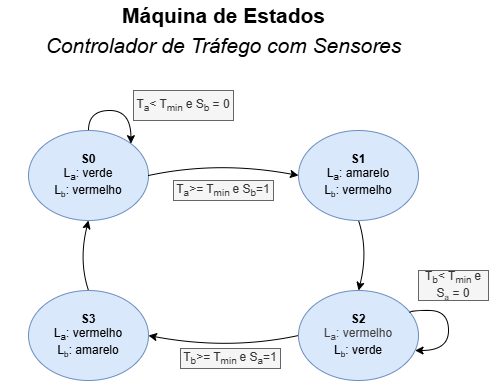
\includegraphics[width=\columnwidth]{maquina-de-estados-sensores.png}
\caption{Circuito da FSM com as entradas dos sensores no Logisim Evolution.}
\label{fig:fsm_sensores}
\end{figure}

\subsection{Pseudocódigo}

O algoritmo síncrono pode ser descrito pelo pseudocódigo a seguir. A variável
\texttt{pulso} é produzida pelo contador e ocorre uma vez a cada oito bordas
de subida do clock.

\begin{lstlisting}[caption={Pseudocodigo da logica de transicao},
label={lst:pseudocodigo}]
se reset = 0 entao
    estado <- S0
senao, a cada borda de subida:
    se pulso = 1 entao
        caso estado de
            S0: se sensor_a = 1 e sensor_b = 0
                    estado <- S0
                senao
                    estado <- S1
            S1: estado <- S2
            S2: se sensor_b = 1 e sensor_a = 0
                    estado <- S2
                senao
                    estado <- S3
            S3: estado <- S0
        fim caso
    fim se
fim
\end{lstlisting}

\subsection{Exemplos de execução}

Considere a sequência inicial S0. Com
\((sensor\_a,sensor\_b)=(0,0)\), o controlador percorre
\(S0\rightarrow S1\rightarrow S2\rightarrow S3\rightarrow S0\).
Com \((1,0)\), S0 permanece ativo enquanto a demanda da via A continuar
exclusiva. Se a FSM estiver em S2 quando a demanda de A aparecer, a
sequência é \(S2\rightarrow S3\rightarrow S0\), respeitando a transição
amarela antes de conceder o verde a A. O caso de prioridade para B é
simétrico. Quando a entrada é \((1,1)\), nenhuma das condições de retenção é
verdadeira e a sequência normal é restaurada.

\section{Arquitetura do Sistema}
\label{sec:arquitetura}

\subsection{Visão geral}

A arquitetura estrutural é composta por cinco blocos principais: contador de
oito clocks, máquina de quatro estados, decodificador de estados,
decodificadores de cores e lógica de habilitação. A Figura~\ref{fig:blocos}
apresenta o diagrama de blocos com os sinais de entrada, a distribuição das
saídas A e B e a integração dos módulos.

\begin{figure}[!t]
\centering
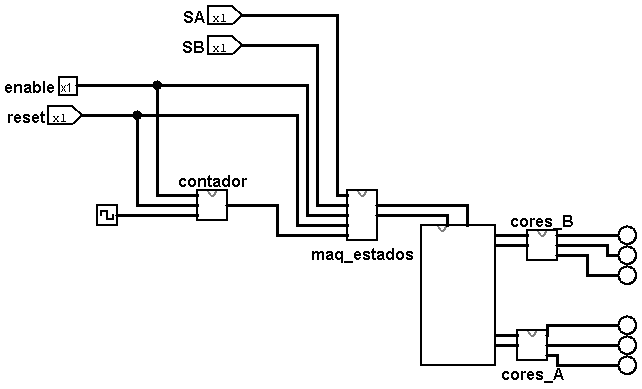
\includegraphics[width=\columnwidth]{main.png}
\caption{Arquitetura integrada do controlador com sensores no Logisim
Evolution.}
\label{fig:blocos}
\end{figure}

O circuito integrado da Figura~\ref{fig:blocos} recebe \texttt{clk},
\texttt{reset}, \texttt{enable}, \texttt{SA} e \texttt{SB}. O bloco
\texttt{contador} divide a frequência de decisão, enquanto
\texttt{maq\_estados} armazena o estado da FSM e recebe os sensores. O
decodificador central distribui o estado para os blocos \texttt{cores\_A} e
\texttt{cores\_B}, que acionam os três LEDs de cada via. Portanto, esta
figura representa a integração efetivamente utilizada, e não somente um
fluxo conceitual.

\subsection{Modelo físico da interseção}

A Figura~\ref{fig:vias} ilustra o cenário de duas vias e a associação
conceitual entre os sensores, os semáforos e os veículos. A imagem não
representa uma implementação elétrica específica do sensor; ela serve para
relacionar os sinais binários do modelo com a situação física que motivou o
algoritmo.

\begin{figure}[!t]
\centering
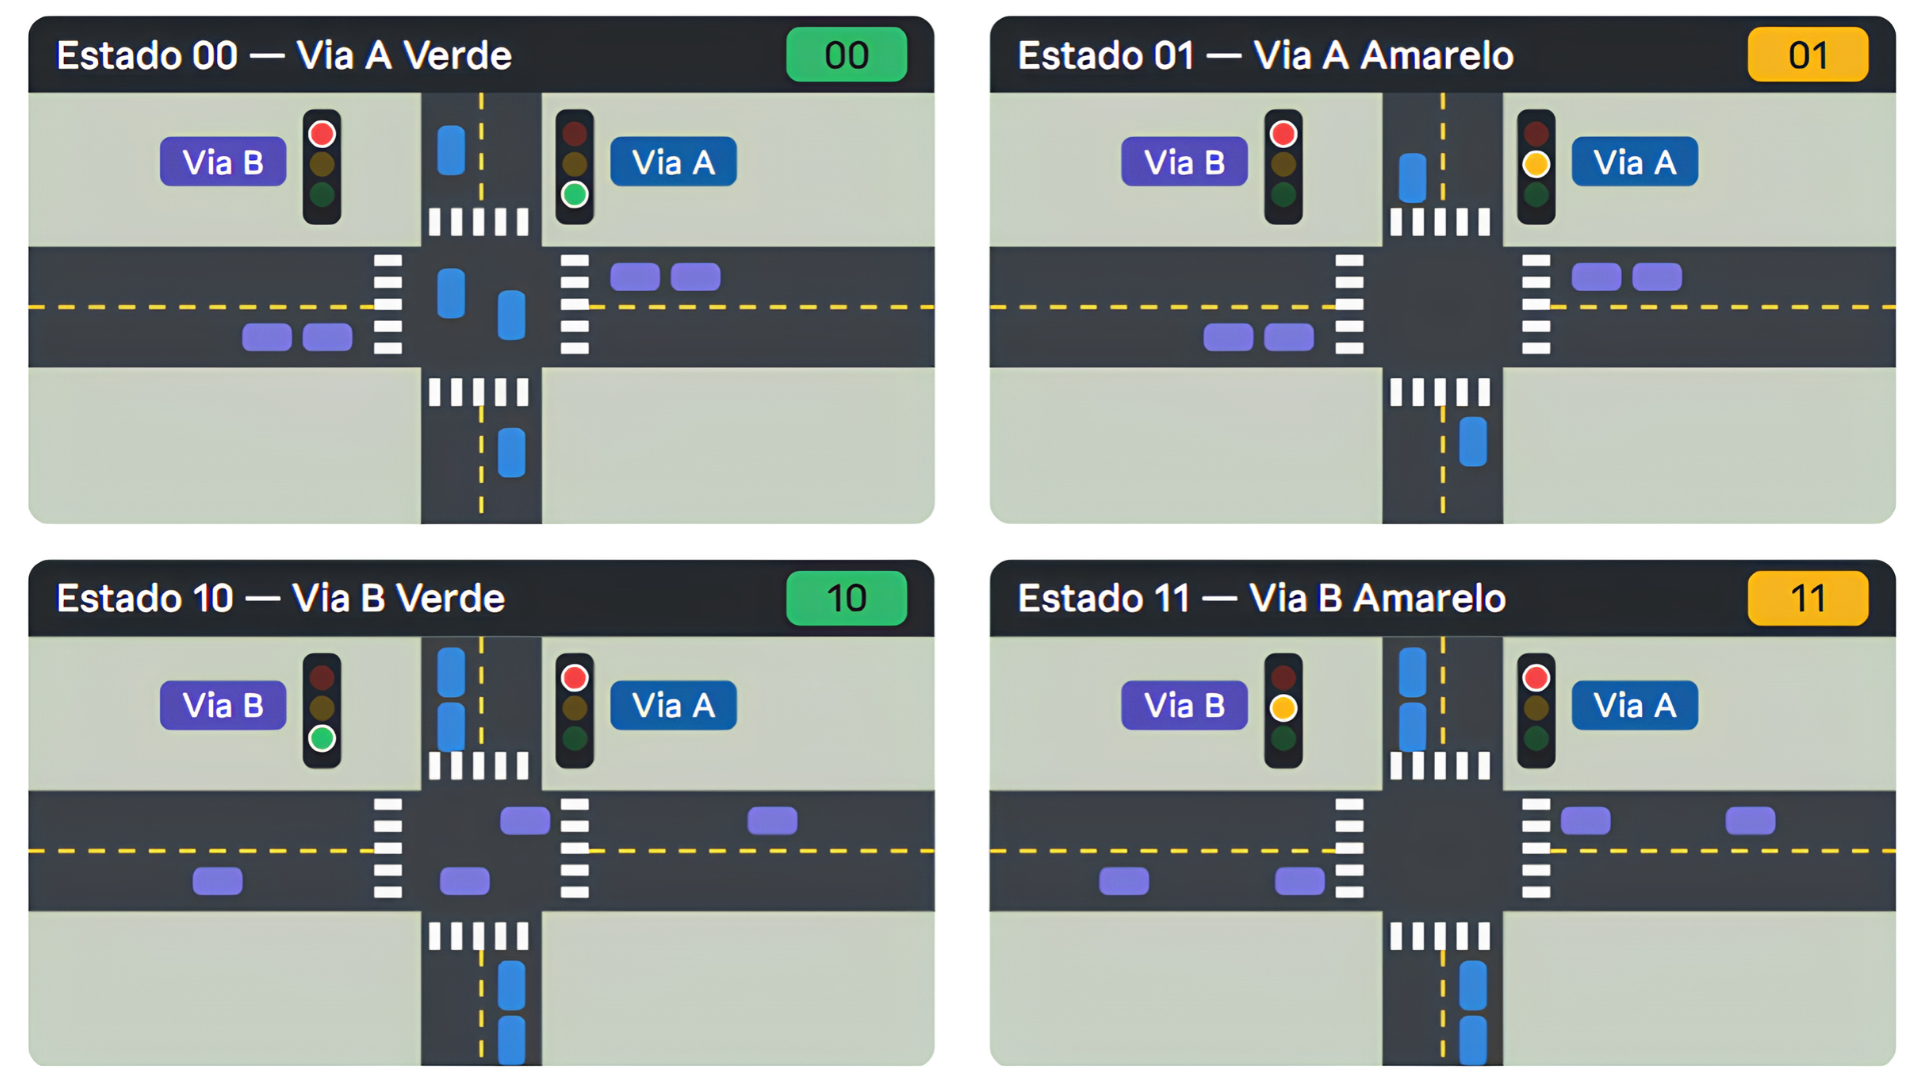
\includegraphics[width=\columnwidth]{esquema-de-vias.png}
\caption{Representação conceitual da interseção com as vias A e B.}
\label{fig:vias}
\end{figure}

\subsection{Codificação das cores}

O decodificador de estados utiliza a codificação apresentada na
Tabela~\ref{tab:codificacao}. Os vetores A e B não são diretamente os seis
LEDs: cada vetor é convertido pelo bloco \texttt{dec\_cores}, que possui
saídas one-hot para vermelho, amarelo e verde.

\begin{table}[!t]
\caption{Codificação dos estados e cores}
\label{tab:codificacao}
\centering
\footnotesize
\begin{tabular}{c|c|c|c}
\toprule
\textbf{Estado} & \textbf{q} & \textbf{Via A} & \textbf{Via B}\\
\midrule
S0 & 00 & verde & vermelho\\
S1 & 01 & amarelo & vermelho\\
S2 & 10 & vermelho & verde\\
S3 & 11 & vermelho & amarelo\\
\bottomrule
\end{tabular}
\end{table}

\subsection{Implementação equivalente em Logisim Evolution}

Antes e durante a validação VHDL, a arquitetura também foi organizada em
blocos no Logisim Evolution. A Figura~\ref{fig:blocos} mostra a integração
principal, incluindo contador, FSM e decodificadores. A
implementação gráfica permite observar as interconexões e verificar a
codificação de estados sem depender apenas do código textual.

O contador mostrado na integração é um divisor temporal de três
bits. Seus flip-flops percorrem os valores de 0 a 7 e a lógica de detecção
do último valor gera o pulso que habilita a FSM. Ele não decide qual via
recebe o verde; sua única função é impor o tempo mínimo de cada fase.

A representação da máquina de estados usada no projeto mostra o circuito sequencial da FSM. As
entradas \texttt{SA} e \texttt{SB} passam por portas lógicas que identificam
as situações de demanda exclusiva. Essas condições são combinadas com o
estado atual, o \texttt{enable} e o \texttt{reset} para formar as entradas
dos flip-flops que armazenam os dois bits de estado.

O decodificador recebe os bits de estado e
gera os códigos destinados aos semáforos A e B. A lógica de saída foi
separada da lógica sequencial para que a troca de cores seja determinada
exclusivamente pela tabela de estados, reduzindo o risco de uma combinação
conflitante.

\subsection{Bloco de contagem no Logisim}

\begin{figure}[!t]
\centering
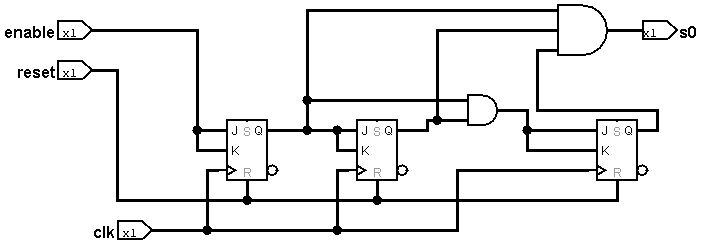
\includegraphics[width=\columnwidth]{cont_8clk.png}
\caption{Contador de oito ciclos implementado no Logisim Evolution.}
\label{fig:logisim_contador}
\end{figure}

O contador é formado por três elementos de memória sincronizados pelo mesmo
clock. Os bits armazenados representam um número entre zero e sete. Uma
combinação de portas detecta o valor final da contagem e gera o sinal
\texttt{S0}, utilizado como pulso de habilitação da máquina. Enquanto esse
pulso não ocorre, a FSM conserva seu estado, mesmo que os sensores mudem.
Essa decisão é importante porque impede que ruídos ou alterações rápidas dos
sensores mudem as cores em toda borda de clock.

Na representação gráfica, o reset limpa os flip-flops do contador e o
\texttt{enable} controla a passagem do clock lógico para o circuito. O bloco
não precisa conhecer as vias A e B: ele é um temporizador independente,
reutilizável para qualquer estado que precise da mesma duração mínima.

\subsection{Máquina de estados no Logisim}

\begin{figure}[!t]
\centering
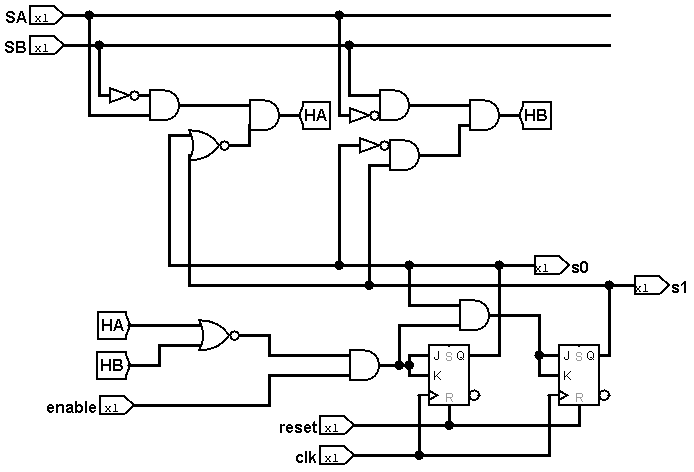
\includegraphics[width=\columnwidth]{maq_estado.png}
\caption{Máquina de estados da via com os sensores \texttt{SA} e \texttt{SB}
no Logisim Evolution.}
\label{fig:logisim_maquina}
\end{figure}

O bloco \texttt{maq\_estados} é o núcleo sequencial do projeto. Seus dois
flip-flops armazenam o vetor \(q[1:0]\), enquanto a lógica combinacional
calcula as condições de retenção e os sinais de entrada dos flip-flops. A
combinação \(SA\overline{SB}\) mantém S0, e a combinação
\(SB\overline{SA}\) mantém S2. Quando os sensores estão iguais, nenhuma
retenção exclusiva é ativada e a sequência normal prossegue.

As entradas \texttt{reset} e \texttt{enable} têm funções diferentes:
\texttt{reset} força o estado inicial seguro, e \texttt{enable} permite que
uma transição calculada seja efetivamente armazenada. Os estados amarelos
não possuem retenção por sensor, pois sua função é intermediar a troca de
uma via para a outra.

\subsection{Decodificador de estados no Logisim}

\begin{figure}[!t]
\centering
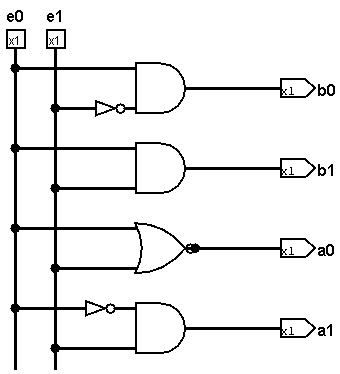
\includegraphics[width=\columnwidth]{dec_estados.png}
\caption{Decodificador dos dois bits de estado no Logisim Evolution.}
\label{fig:logisim_dec_estados}
\end{figure}

O decodificador recebe \(q_1\) e \(q_0\) e produz dois códigos de dois bits,
um para cada via. As portas AND e OR implementam diretamente a tabela
apresentada na Tabela~\ref{tab:codificacao}. Por exemplo, em S0 o circuito
produz o código de verde para A e o código de vermelho para B; em S2, a
associação é invertida. Como o bloco não possui memória, suas saídas mudam
imediatamente após a estabilização dos bits da FSM.

\subsection{Decodificador de cores no Logisim}

\begin{figure}[!t]
\centering
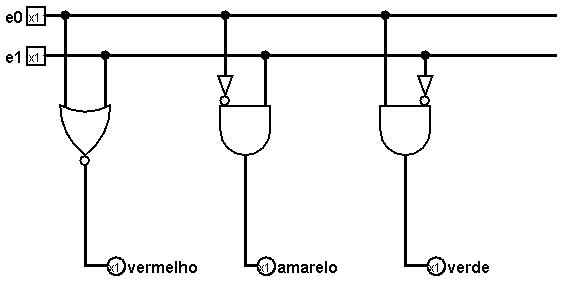
\includegraphics[width=\columnwidth]{dec_cores.png}
\caption{Decodificador de cores das vias no Logisim Evolution.}
\label{fig:logisim_dec_cores}
\end{figure}

O decodificador de cores é replicado para cada via. Ele recebe o código
produzido pelo decodificador de estados e aciona três saídas, uma para cada
cor. A implementação usa portas inversoras, AND e OR para gerar as funções
de vermelho, amarelo e verde. O uso de um mesmo bloco para A e B reduz a
duplicação e garante que as duas vias obedeçam à mesma convenção elétrica.

\subsection{Integração dos circuitos no Logisim}

Na integração, o pulso do contador é combinado com \texttt{enable} antes de
chegar à FSM. O vetor de estado segue para o decodificador de estados e é
duplicado em dois caminhos, um para cada decodificador de cores. Os sensores
entram somente no circuito da FSM; portanto, não há caminho combinacional
direto dos sensores para os LEDs. Essa característica mantém as saídas
associadas a estados válidos e facilita a comparação com a forma de onda
VHDL.

\section{Implementação em VHDL}
\label{sec:vhdl}

\subsection{Organização hierárquica}

O projeto é dividido nos arquivos \texttt{contador\_8clk.vhd},
\texttt{maq\_4estados.vhd}, \texttt{dec\_4estados.vhd},
\texttt{dec\_cores.vhd}, \texttt{design.vhd} e \texttt{testbench.vhd}.
Essa decomposição mantém no nível superior somente as conexões entre
componentes e deixa cada decisão funcional em um módulo específico.

O arquivo \texttt{design.vhd} instancia os módulos por meio de
\texttt{entity work.nome\_do\_modulo}, formando uma arquitetura estrutural.
O uso de \texttt{std\_logic} e \texttt{std\_logic\_vector} é compatível com
a biblioteca IEEE \texttt{std\_logic\_1164}, que oferece tipos resolvidos e
operações lógicas apropriadas para sinais digitais \cite{ieee1076,ieee1164}.

\subsection{Módulo \texttt{contador\_8clk.vhd}}

O módulo VHDL equivalente ao contador usa um sinal inteiro com faixa
\texttt{0 to 7}. A restrição de faixa documenta a largura funcional do
contador e permite que a ferramenta detecte atribuições fora do intervalo.
Dentro de um processo sensível a \texttt{clk}, a borda de subida incrementa
o valor; quando o valor é 7, o contador retorna a zero e atribui '1' à saída
\texttt{saida}. Em qualquer outra contagem, \texttt{saida} recebe '0'.

O contador possui, portanto, a mesma função do circuito Logisim:
transformar oito bordas de clock em um pulso de habilitação. Em um clock de
período \(T_{clk}\), a duração nominal entre pulsos é
\begin{equation}
T_{\min}=8T_{clk}.
\label{eq:tmin}
\end{equation}

No testbench, \(T_{clk}=20\)~ns, logo \(T_{\min}=160\)~ns. O contador não
altera diretamente as cores; ele somente limita a frequência com que a FSM
pode mudar de estado. Essa separação corresponde ao contador formado por
flip-flops no Logisim e permite substituir o clock de simulação por outro
clock sem modificar a tabela de estados.

\subsection{Módulo \texttt{maq\_4estados.vhd}}

A FSM é descrita por um processo sensível a \texttt{clk} e \texttt{clrn},
correspondendo aos flip-flops do circuito Logisim. O reset assíncrono força
S0, estado que deixa a via A verde e a via B vermelha. Em uma borda de
subida, a máquina somente avalia uma transição quando
\texttt{ena\_estado} está em nível alto. Assim, a atribuição ao sinal
\texttt{estado} representa a atualização dos elementos de memória, e não
uma lógica combinacional.

O trecho essencial da retenção de prioridade é:

\begin{lstlisting}[caption={Trecho da FSM para a prioridade da via A},
label={lst:fsm}]
when "00" =>
    if sensor_a = '1' and sensor_b = '0' then
        estado <= "00";
    else
        estado <= "01";
    end if;
\end{lstlisting}

O trecho equivalente para S2 usa a condição
\texttt{sensor\_b = '1' and sensor\_a = '0'}. A exigência das duas
condições, e não de apenas um sensor, é o que garante que a presença de
veículos nas duas vias não bloqueie a alternância normal.

\subsection{Módulo \texttt{dec\_4estados.vhd}}

O módulo \texttt{dec\_4estados} implementa, em VHDL, as portas
combinacionais do decodificador gráfico. O vetor \texttt{estado} é utilizado
como seletor de um comando \texttt{case}; para cada um dos quatro códigos,
o processo atribui simultaneamente os vetores A e B. Dessa forma, o módulo
não armazena informação e apenas traduz a codificação da FSM.

O uso de atribuições em todos os ramos do \texttt{case} evita que A ou B
retenham valores de uma combinação anterior. A equivalência com o Logisim
é direta: as expressões booleanas implementadas por portas são agrupadas no
comando de seleção, mas a tabela de conversão permanece a mesma.

\subsection{Módulo \texttt{dec\_cores.vhd}}

O módulo \texttt{dec\_cores} é instanciado duas vezes no arquivo superior,
uma vez para A e outra para B. Ele recebe um vetor de dois bits e produz
\texttt{vermelho}, \texttt{amarelo} e \texttt{verde}. O código 01 representa
amarelo, o código 10 representa verde e os demais códigos resultam em
vermelho. Esse último ramo também define uma saída segura para códigos não
utilizados.

O processo combinacional é equivalente ao circuito de portas do decodificador
gráfico do projeto. Como as duas instâncias usam exatamente o
mesmo módulo, a implementação em VHDL preserva a simetria visual do
Logisim e reduz a possibilidade de uma via usar uma codificação diferente.

\subsection{Módulo superior \texttt{design.vhd}}

O arquivo \texttt{design.vhd} realiza a integração estrutural. Ele instancia
o contador, calcula \texttt{ena\_estado}, instancia a FSM, conecta o
decodificador de estados e, por fim, instancia os dois decodificadores de
cores. Os sinais \texttt{sensor\_a} e \texttt{sensor\_b} são conectados
diretamente às portas correspondentes da FSM, enquanto as saídas A e B são
conectadas às instâncias de cores.

Essa organização é a mesma mostrada na Figura~\ref{fig:blocos}: os módulos
possuem responsabilidades separadas e as conexões ficam no nível superior.
Consequentemente, uma alteração no temporizador não exige modificar os
decodificadores, e uma alteração na codificação das cores não exige
reescrever a lógica de prioridade.

\subsection{Decodificação e segurança das saídas}

O decodificador de estados associa S0 a A verde/B vermelho, S1 a A
amarelo/B vermelho, S2 a A vermelho/B verde e S3 a A vermelho/B amarelo.
O segundo decodificador transforma cada código de dois bits em três sinais
de saída. Como cada estado válido contém apenas uma indicação verde e uma
indicação amarela, o modelo evita a condição de dois verdes simultâneos.

Os processos combinacionais possuem o estado como única entrada e atribuem
valores às saídas em todos os ramos do \texttt{case}. Isso evita retenção
acidental de valores e torna explícita a relação entre o código da FSM e as
cores observáveis.

\subsection{Testbench}

O testbench gera um clock de 20~ns, mantém o reset ativo inicialmente,
habilita o controlador e percorre quatro situações: nenhum sensor ativo,
somente A ativa, somente B ativa e ambas ativas. O arquivo de ondas é gerado
com GHDL, ferramenta de simulação VHDL baseada em GCC e LLVM
\cite{ghdlmanual}. A análise pode ser repetida com:

\begin{lstlisting}[caption={Comandos de compilacao e simulacao},
label={lst:ghdl}]
ghdl -a contador_8clk.vhd dec_4estados.vhd dec_cores.vhd \
  maq_4estados.vhd design.vhd testbench.vhd
ghdl -e tb_semaforo
ghdl -r tb_semaforo --vcd=wave.vcd --stop-time=1200ns
\end{lstlisting}

\section{Resultados de Simulação}
\label{sec:resultados}

\subsection{Forma de onda geral}

A Figura~\ref{fig:wave} apresenta a forma de onda registrada no GTKWave.
Durante os primeiros 100~ns, \texttt{clrn} permanece em zero e o estado
mantém a codificação 00. Depois da liberação do reset, a sequência inicial
passa por 01 e 10, ativando respectivamente o amarelo de A e o verde de B.
Cada transição ocorre alinhada ao pulso produzido pelo contador de oito
clocks.

\begin{figure*}[!t]
\centering
\includegraphics[width=0.96\textwidth]{simulador-de-ondas.png}
\caption{Forma de onda da simulação VHDL observada no GTKWave.}
\label{fig:wave}
\end{figure*}

\subsection{Análise dos cenários}

Na região inicial em que \texttt{sensor\_a} e \texttt{sensor\_b} estão em
zero, os estados alternam de forma periódica. Isso confirma o caso de
operação normal. Quando somente \texttt{sensor\_a} é elevado, a FSM pode
permanecer em S0, mantendo \texttt{verde\_a} ativo e \texttt{vermelho\_b}
ativo. A mudança para A acontece sem eliminar a fase amarela quando o
controlador estava anteriormente em S2.

Na etapa seguinte, o testbench desativa A e ativa somente B. A FSM abandona
S0 pela transição S1 e chega a S2, concedendo o verde à via B. Quando A é
ativada novamente enquanto B continua ativa, as condições de exclusividade
deixam de ser verdadeiras; o controlador volta a alternar pelos quatro
estados. Esse último caso verifica diretamente o requisito de que veículos
nas duas vias não devem produzir retenção indefinida.

\begin{table}[!t]
\caption{Casos de teste e resultado observado}
\label{tab:testes}
\centering
\footnotesize
\begin{tabular}{c|c|p{0.42\columnwidth}}
\toprule
\textbf{Caso} & \textbf{Sensores} & \textbf{Resultado}\\
\midrule
1 & 00 & Sequência S0--S1--S2--S3.\\
2 & 10 & Retenção em S0 quando A já está verde.\\
3 & 01 & Transição para S2 após a fase amarela.\\
4 & 11 & Alternância normal restaurada.\\
\bottomrule
\end{tabular}
\end{table}

\subsection{Comparação com o modelo gráfico}

As imagens do Logisim confirmam a correspondência entre a codificação de
dois bits e as cores dos semáforos. O decodificador de cores utilizado no
modelo ativa uma única lâmpada para cada combinação válida. Essa verificação
complementar é útil porque o modelo
gráfico evidencia visualmente as conexões que no VHDL aparecem como
associações de portas.

O circuito do decodificador de cores recebe os dois bits associados a uma via.
Ele implementa as funções
combinacionais que acionam vermelho, amarelo ou verde. Para cada código
válido, exatamente uma saída permanece ativa; assim, o bloco converte a
representação compacta da FSM em sinais diretamente conectáveis aos LEDs.

\section{Discussão}
\label{sec:discussao}

O algoritmo satisfaz a política de prioridade solicitada sem criar uma
transição insegura. A decisão é tomada somente nos instantes de
habilitação e a troca entre vias sempre passa por um estado amarelo. A
organização modular também permite substituir sensores ideais por circuitos
de condicionamento ou sincronização sem alterar os decodificadores.

Há, entretanto, uma limitação comportamental importante: quando apenas uma
via possui veículos, seu estado verde pode ser mantido indefinidamente. Essa
decisão é coerente com a prioridade ``se possível'', mas não implementa
justiça temporal nem um tempo máximo de atendimento. Em uma aplicação real,
seria necessário adicionar um segundo contador, um parâmetro de tempo máximo
ou uma política de aging para impedir starvation da via oposta.

Também se assume que os sensores chegam sincronizados ao clock. Sensores
físicos podem apresentar ruído, bouncing ou mudanças próximas à borda de
clock. Uma versão de hardware deveria incluir sincronizadores de dois
flip-flops, filtragem e, eventualmente, detecção de presença persistente.
Esses elementos estão fora do escopo do modelo didático, mas são relevantes
para a síntese em FPGA ou ASIC.

\section{Conclusão}
\label{sec:conclusao}

Foi desenvolvido um controlador de tráfego de duas vias em VHDL, baseado em
uma FSM de quatro estados, contador de oito clocks e decodificadores
hierárquicos. A especificação foi traduzida para quatro cenários: operação
normal sem veículos, prioridade exclusiva para A, prioridade exclusiva para
B e alternância normal quando as duas vias estão ocupadas.

Os resultados de simulação confirmaram que os estados e as cores dos
semáforos seguem a arquitetura planejada. Com clock de 20~ns, cada fase
possui duração mínima de 160~ns, enquanto o ciclo completo sem retenção
possui 640~ns. A comparação com os blocos do Logisim Evolution reforçou a
correspondência entre a implementação estrutural e o comportamento VHDL.

As principais dificuldades foram organizar as transições condicionais sem
comprometer as fases amarelas e manter a coerência entre diagramas,
decodificadores e sinais de onda. Como melhorias, destacam-se a inclusão de
tempo máximo configurável, sincronização dos sensores, filtros de entrada,
assertions no testbench e testes automatizados para todas as combinações de
sensores. Dessa forma, o algoritmo apresentado pode evoluir de um modelo
didático para um controlador digital sintetizável com requisitos temporais
mais próximos de uma aplicação real.

\begin{thebibliography}{10}

\bibitem{ieee1076}
IEEE Standards Association, ``IEEE Standard for VHDL Language Reference
Manual,'' IEEE Std 1076-2019, 2019.

\bibitem{ieee1164}
IEEE Standards Association, ``IEEE Standard Multivalue Logic System for VHDL
Model Interoperability,'' IEEE Std 1164-1993, 1993.

\bibitem{ashenden2008}
P. J. Ashenden, \emph{The Designer's Guide to VHDL}, 3rd ed.
San Francisco, CA, USA: Morgan Kaufmann, 2008.

\bibitem{brown2015}
S. Brown and Z. Vranesic, \emph{Fundamentals of Digital Logic with VHDL
Design}, 3rd ed. New York, NY, USA: McGraw-Hill, 2015.

\bibitem{wakerly2018}
J. F. Wakerly, \emph{Digital Design: Principles and Practices}, 5th ed.
Boston, MA, USA: Pearson, 2018.

\bibitem{harris2021}
D. M. Harris and S. L. Harris, \emph{Digital Design and Computer
Architecture: RISC-V Edition}. Cambridge, MA, USA: Morgan Kaufmann, 2021.

\bibitem{ghdlmanual}
T. Gingold et al., ``GHDL user manual,'' GHDL Project, 2024. [Online].
Available: \url{https://ghdl.github.io/ghdl/}

\bibitem{stdlogic}
IEEE, ``IEEE packages and standard logic types for VHDL,'' IEEE Standards
Association. [Online]. Available:
\url{https://standards.ieee.org/standard/1164-1993.html}

\bibitem{logisim}
B. L. D. Joshi et al., ``Logisim Evolution,'' open-source digital logic
simulator, 2024. [Online]. Available:
\url{https://github.com/logisim-evolution/logisim-evolution}

\bibitem{ieeetran}
M. Shell, ``IEEEtran class documentation,'' IEEEtran project, 2015.
[Online]. Available: \url{https://www.ctan.org/pkg/ieeetran}

\bibitem{vhdlguide}
D. L. Perry, \emph{VHDL: Programming by Example}, 4th ed. New York, NY,
USA: McGraw-Hill, 2002.

\end{thebibliography}

\end{document}
